\section{Experiment}
\label{Section: experiment}

\subsection{Datasets}
\textcolor{note}{this section is too long}

Due to most of public sources datasets cannot fully satisfy all configuration choices, for example, some can only guarantee 30 frames but cannot guarantee 1024p resolution, while others can guarantee resolution but cannot provide sufficient frame rate, but in recent years, most of the driving recorder can provide enough resolution and frame rate, so we try to use Youtube video as fellows. First, in order to eliminate the bias caused by Cookies and personal preferences, we use private browsing mode to search keywords (e.g., "drivecam highway hd"). Second, manually delete irrelevant videos (e.g., ads for some driving recorders) and download videos that are longer than ten minutes. In addition, these videos need to be as dynamic as the real world, such as not standing still for too long. Becaues of none of these videos contained ground truth, we used the data of the original video output from DNN as the tags to calculate the accuracy. For instance, in object detection, the accuracy is defined by the F1 score with respect to the server-side DNN output in highest resolution (original) with over 50$\%$ confidence score.Based on the above filtering strategy, we finally selected three datasets: 

M6: The M6 is the longest motorway in Britain and the most important road from the Midlands to the West Coast. Thousands of cars travel on it every day. This video was taken from a traffic camera, and its natural dynamics allows us to experiment with this video.

Duke: Duke is a video from a fixed camera placed at an intersection. Because it is fixed in the middle of the intersection, the traffic flow in the video increases or decreases periodically as the traffic light change.

Mutli Camera Dataset: Since the first two datasets were sourced from a fixed camera, in order to ensure that AutoConfigure still has better performance when road conditions change dramatically, we used three videos collected from the dashcam, and since they are relatively similar, we combined them into one video.

\begin{figure*}[!t]
	\begin{minipage}[t]{0.32\linewidth}
		\centerline{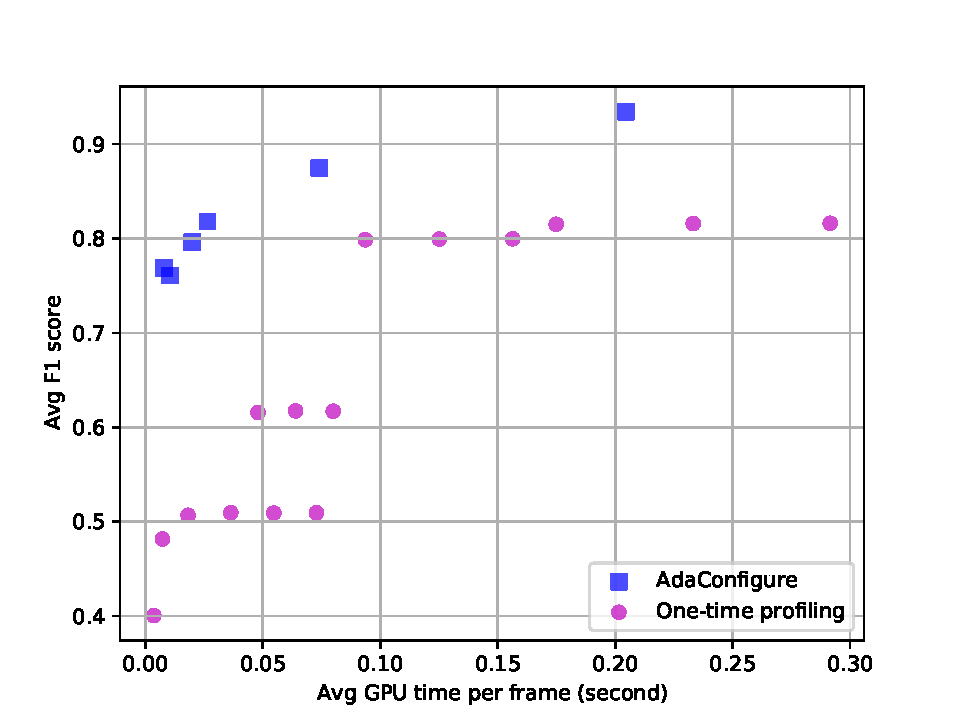
\includegraphics[width=6.5cm]{figures/m6.pdf}}
		\centerline{(a) M6}
	\end{minipage}
	\hfill
	\begin{minipage}[t]{0.32\linewidth}
		\centerline{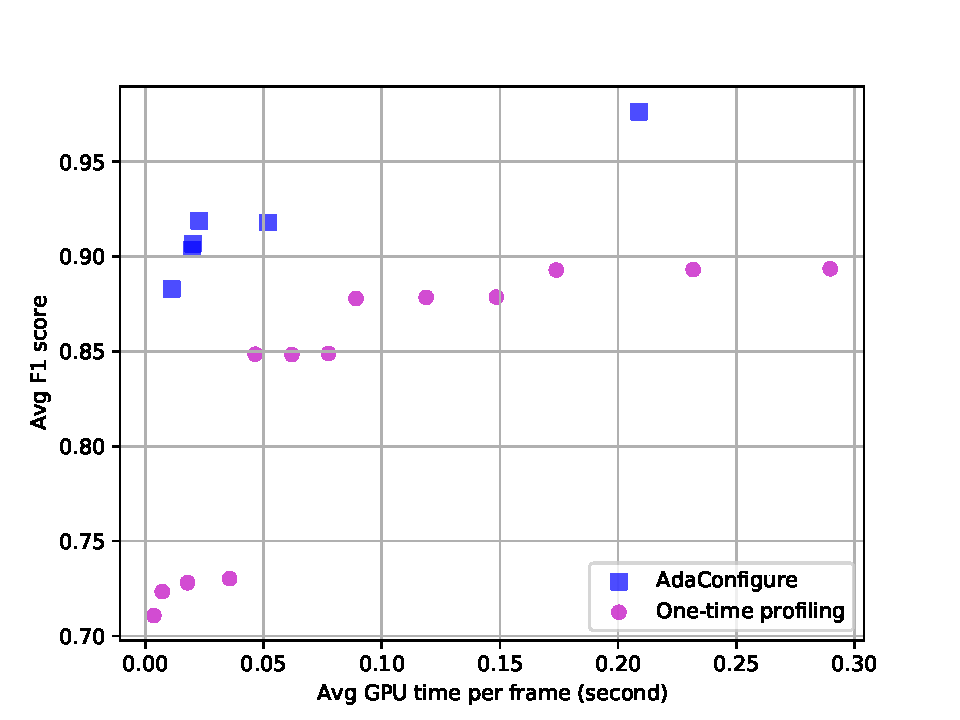
\includegraphics[width=6.5cm]{figures/duke.pdf}}
		\centerline{(b) Duke}
	\end{minipage}
	\hfill
	\begin{minipage}[t]{0.32\linewidth}
		\centerline{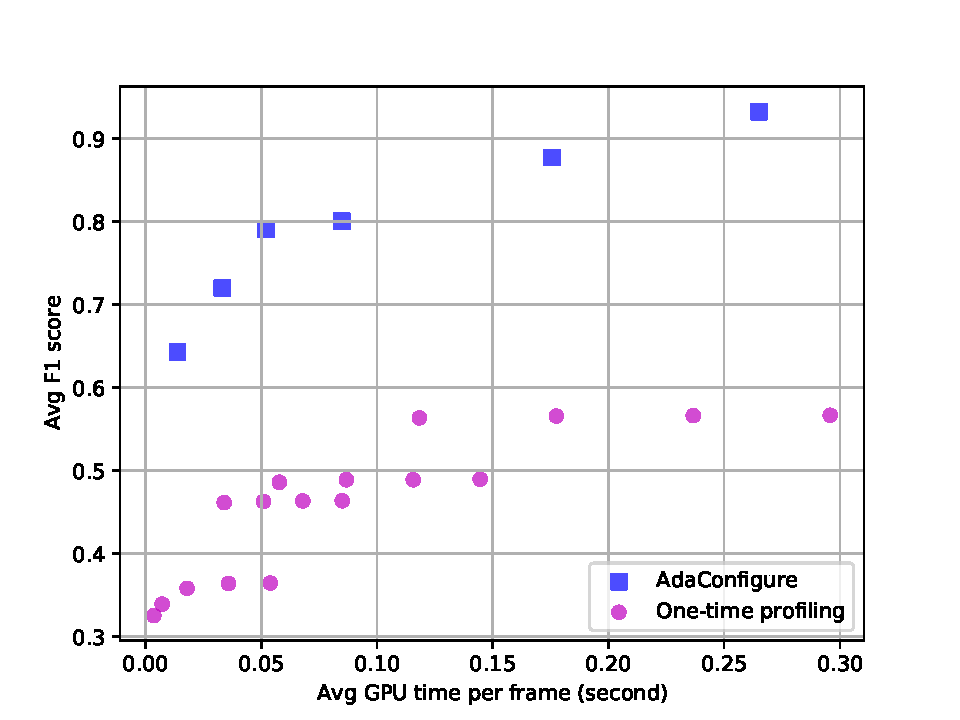
\includegraphics[width=6.5cm]{figures/_Westbound_Eastbound_Rear.pdf}}
		\centerline{(c) Multi Camera Dataset}
	\end{minipage}		
	\caption{The effect of different models, frame rate, and resolutions on accuracy and processing time. AutoConfigure (blue) consistently outperforms the baseline of one-time update (magenta) across different datasets. Each dot represents the results of running each solution.}
	\label{fig_results}
\end{figure*}

\subsection{Configure Selection}
We simulate the environment with three object detection models, which are SSD ResNet152V1, FasterRCNN ResNet50V1, FasterRCNN InceptionResNetV2. For each model, two kinds of image resolution for inference, which is $1024\times1024$ and $640\times640$, can be picked up. Besides choosing a proper configure of model and image resolution, AutoConfigure needs to select a proper number of frames per second(fps). We in our experiment, we set the choices space of fps as \{1, 2, 5, 10, 15, 20, 25, 30\}. Therefore, the number of actions that the agent can choose is forty-eight.
\subsection{Experiment Parameters}
We apply deep Q-learning policy to train the agent. In the training procedure, we build up eight independently identical environments for each data set to speed up the training and decrease the dependency of the data. The leaning rate is set to 0.001. The discount factor is set to 0.9. For each dataset, we train the agent 10 epochs and 1000 steps per epoch. The exploration factor is 0.9. The inference models are implemented in Tensorflow and are pretrained on standard image datasets \cite{trade-offs}, and the switching of video frame rate and resolution is done by FFmpeg \cite{ffmpeg}.
\subsection{Experiment Results}

%\begin{table}[!t]
%%\begin{table}[H]
%	\centering
%	%     \begin{tabular}{lll}
%	\resizebox{0.5\textwidth}{!}{
%		\begin{tabular}{lcc}
%			\toprule
%			Model and Image size & Inference time & Accuracy  \\ \midrule
%			SSD MobileNetV2 320p          & 49.5 ms  &  xxx            \\
%			SSD MobileNetV2 640p          & 58.5 ms  &  0.494            \\
%			SSD ResNet152V1 640p          & 100 ms  &  0.579            \\
%			SSD ResNet152V1 1024p          & 182.3 ms  &  0.614            \\
%			FasterRCNN ResNet50V1 640p          & 106.4 ms  &  0.637            \\
%			FasterRCNN ResNet50V1 1024p          & 120.5 ms  &  0.786           \\
%			FasterRCNN InceptionResNetV2 640p          & 361.8 ms  &  0.734            \\
%			FasterRCNN InceptionResNetV2 1024p          & 418.4 ms  &  1            \\
%			\bottomrule
%	\end{tabular}}
%	\caption{Inference time and F1 for different models and resolutions car truck}
%	\label{tab: latency-overhead}
%	% \vspace{-0.5cm}
%\end{table}
%
%\begin{table}[!t]
%	%\begin{table}[H]
%	\centering
%	%     \begin{tabular}{lll}
%	\resizebox{0.5\textwidth}{!}{
%		\begin{tabular}{lcc}
%			\toprule
%			Model and Image size & Inference time & Accuracy  \\ \midrule
%			SSD MobileNetV2 320p          & 49.5 ms  &  xxx            \\
%			SSD MobileNetV2 640p          & 58.5 ms  &  0.753            \\
%			SSD ResNet152V1 640p          & 100 ms  &  0.886            \\
%			SSD ResNet152V1 1024p          & 182.3 ms  &  0.942            \\
%			FasterRCNN ResNet50V1 640p          & 106.4 ms  &  0.889            \\
%			FasterRCNN ResNet50V1 1024p          & 120.5 ms  &  0.98           \\
%			FasterRCNN InceptionResNetV2 640p          & 361.8 ms  &  0.965            \\
%			FasterRCNN InceptionResNetV2 1024p          & 418.4 ms  &  1            \\
%			\bottomrule
%	\end{tabular}}
%	\caption{Inference time and F1 for different models and resolutions}
%	\label{tab: latency-overhead}
%	% \vspace{-0.5cm}
%\end{table}

%\begin{figure}[!t]
%	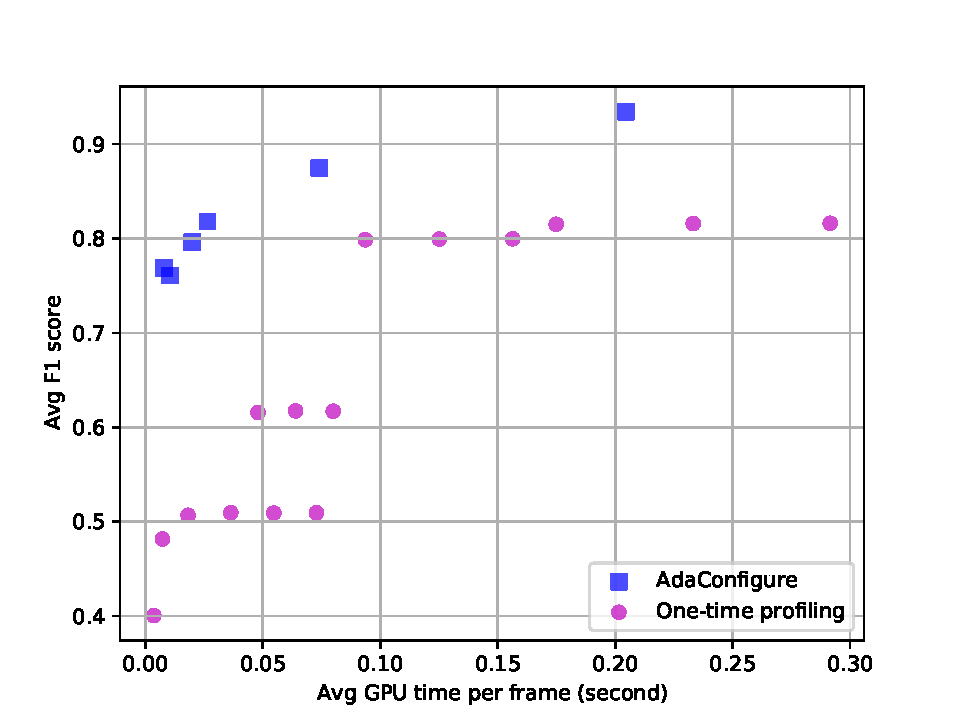
\includegraphics[width=9cm,height=8cm]{figures/m6.pdf}
%	\centering
%	\caption{The effect of different models, frame rate, and resolutions on accuracy and processing time. AutoConfigure (blue) consistently outperforms the baseline of one-time update (magenta) across different datasets. Each dot represents the results of running each solution.}
%	\label{fig_m6}
%\end{figure}